\documentclass{sbc2023}%
\usepackage{float}
\usepackage{graphicx}
%\usepackage[utf8]{inputenc}
\usepackage[misc,geometry]{ifsym} 
\usepackage{fontspec}
\usepackage{fontawesome}
\usepackage{academicons}
\usepackage{color}
\usepackage{hyperref} 
\usepackage{aas_macros}
\usepackage[bottom]{footmisc}
\usepackage{supertabular}
\usepackage{afterpage}
\usepackage{url}
\usepackage{pifont}
\usepackage{multicol}
\usepackage{multirow}

\documentclass{article}
\usepackage[backend=biber,style=numeric,giveninits=true]{biblatex}
\addbibresource{refs.bib}
\usepackage{hyperref}

\setcitestyle{square}

\definecolor{orcidlogo}{rgb}{0.37,0.48,0.13}
\definecolor{unilogo}{rgb}{0.16, 0.26, 0.58}
\definecolor{maillogo}{rgb}{0.58, 0.16, 0.26}
\definecolor{darkblue}{rgb}{0.0,0.0,0.0}
\hypersetup{colorlinks,breaklinks,
            linkcolor=darkblue,urlcolor=darkblue,
            anchorcolor=darkblue,citecolor=darkblue}
%\hypersetup{colorlinks,citecolor=blue,linkcolor=blue,urlcolor=blue}

%%%%%%% IMPORTANT: We disable hyperlinks by default with this line, to avoid the error "\pdfendlink ended up in different nesting level" while writing.
%\hypersetup{draft}

\jid{JBCS}
\jtitle{Journal of the Brazilian Computer Society, 2025, XX:1, }
\doi{10.5753/jbcs.2025.XXXXXX}
\copyrightstatement{This work is licensed under a Creative Commons Attribution 4.0 International License}
\jyear{2025}


\title[Presenting the JBCS template]{Enumeration of Cycles in an Undirected Graph}

%THE ORCID IS MANDATORY FOR EACH AUTHOR IN JBCS
\author[Viterbo et al. 2025]{
\affil{\textbf{Felipe Vilhena Dias}~\href{https://orcid.org/my-orcid?orcid=0009-0001-3195-1605}{\textcolor{orcidlogo}{\aiOrcid}}~\textcolor{blue}{\faEnvelopeO}~~[~\textbf{Pontifical University Catholical of Minas Gerais}~|\href{mailto:felipe.dias.1466692@sga.pucminas.br}{~\textbf{\textit{felipe.dias.1466692@sga.pucminas.br}}}~]}

\affil{\textbf{Arthur Clemente Machado}~\href{https://orcid.org/0000-0002-7110-2026}{\textcolor{orcidlogo}{\aiOrcid}}~~[~\textbf{Pontifical University Catholical of Minas Gerais}~|\href{mailto:arthur.clemente@sga.pucminas.br}{~\textbf{\textit{arthur.clemente@sga.pucminas.br}}}~]}

\affil{\textbf{Lucas Henrique Rocha Hauck}~\href{https://orcid.org/0000-0003-3052-3016}{\textcolor{orcidlogo}{\aiOrcid}}~~[~\textbf{Pontifical University Catholical of Minas Gerais}~|\href{mailto:lhauck@sga.pucminas.br}{~\textbf{\textit{lhauck@sga.pucminas.br}}}~]}

\affil{\textbf{Luan Barbosa Rosa Carrieiros}~\href{https://orcid.org/0000-0002-2431-8457}{\textcolor{orcidlogo}{\aiOrcid}}~~[~\textbf{Pontifical University Catholical of Minas Gerais}~|\href{mailto:luan.rosa@sga.pucminas.br}{~\textbf{\textit{luan.rosa@sga.pucminas.br}}}~]}

\affil{\textbf{Diego Moreira Rocha}~\href{https://orcid.org/0000-0002-2431-8457}{\textcolor{orcidlogo}{\aiOrcid}}~~[~\textbf{Pontifical University Catholical of Minas Gerais}~|\href{mailto:diego.moreira@sga.pucminas.br}{~\textbf{\textit{diego.moreira@sga.pucminas.br}}}~]}

\affil{\textbf{Iago Fereguetti Ribeiro}~\href{https://orcid.org/0000-0002-2431-8457}{\textcolor{orcidlogo}{\aiOrcid}}~~[~\textbf{Pontifical University Catholical of Minas Gerais}~|\href{mailto:iago.fereguetti@sga.pucminas.br}{~\textbf{\textit{iago.fereguetti@sga.pucminas.br}}}~]}
}

\begin{document}

\begin{frontmatter}
\maketitle

\begin{mail}
PUC Minas, Instituto de Ciências Exatas e Informática (ICEI), Av. Dom José Gaspar, 500, Coração Eucarístico, Belo Horizonte, MG, 30535-901, Brazil.
\end{mail}

\begin{abstract}
\textbf{Abstract.~}
\noindent This work addresses the problem of enumerating cycles in undirected simple graphs, utilizing two distinct approaches: \textbf{(i)} a permutation-based method and \textbf{(ii)} a graph traversal-based method. The first technique explores vertex permutations to identify cycles, while the second uses graph traversal algorithms to detect closed paths. Both approaches were implemented, and a comparative analysis was conducted to evaluate their performance, particularly as the graph size increases. The experiments highlight the advantages and limitations of each method, and the choice of graph representation is justified. Additionally, the applicability of the solutions to directed graphs is discussed, evaluating the feasibility of the implementations in that context.
\end{abstract}

\begin{keywords}
Cycle enumeration,
Undirected graph,
Graph traversal,
Permutation-based method,
Cycle detection,
Performance analysis,
Graph representation,
Directed graphs,
\end{keywords}

%\begin{license}
%Published under the Creative Commons Attribution 4.0 International Public License (CC BY 4.0)
%\end{license}

\end{frontmatter}


\section{Introduction}
\label{sec:intro}

Graph cycle enumeration is a fundamental problem in graph theory with applications in various domains such as network analysis, biology, circuit design, and social network analysis. Identifying cycles in a graph can help detect feedback loops in circuits, analyze ecosystem structures in biology, and even recognize fraudulent activities in financial networks. The goal of this study is to compare two different approaches for cycle enumeration in undirected graphs: one based on vertex permutation and another utilizing traversal techniques.

While the permutation-based approach systematically generates all possible orderings of vertices, the traversal-based approach employs depth-first search \textbf{(DFS)} to detect cycles efficiently. By implementing and analyzing both methods, we aim to determine their strengths, weaknesses, and practical usability in different scenarios.
 
\section{Graph Representation}
A graph can be represented in multiple ways, each impacting the efficiency of different algorithms. In our implementation, we utilize two distinct data structures to represent graphs:

\textbf{Adjacency Matrix:} Used in the traversal-based approach, this representation provides quick access to edge information but consumes more memory for sparse graphs.

\textbf{Adjacency List:} Used in the permutation-based approach, this structure is more memory-efficient and better suited for graphs with fewer edges.

These representations influence memory usage and computational complexity, affecting overall algorithm performance. The choice of representation is a crucial factor in determining which method is better suited for a given problem instance.

\section{Methodology}
\subsection{Team Roles and Contributions}
Each team member was responsible for creating two codes in different programming languages using different data structures: one code using permutation and the other using traversal. With this approach, we were able to compare various scenarios and determine the most efficient method.

In C, Diego Moreira worked on the adjacency list, Lucas Henrique Hauck on the adjacency matrix, and Luan Barbosa on dual lists for the permutation approach. For traversal in C, Iago Fereguetti handled the adjacency list, Arthur Clemente the adjacency matrix, and Felipe Vilhena the dual lists. In C++, Felipe Vilhena implemented the adjacency list, Iago Fereguetti the adjacency matrix, and Arthur the dual lists for permutation, while Luan Barbosa, Diego Moreira, and Lucas Henrique Hauck focused on the adjacency list, adjacency matrix, and dual lists, respectively, for traversal.

\subsection{Permutation-Based Approach}

The permutation-based approach relies on generating all possible vertex orderings and checking whether they form valid cycles. The key steps include:

Generating all possible permutations of graph vertices.

Checking each permutation to determine if it forms a valid cycle by verifying that consecutive vertices are connected by edges and that the sequence returns to the starting vertex.

Avoiding duplicate cycles using a set-based structure to ensure uniqueness.

This method provides an exhaustive way to identify cycles but becomes computationally expensive as the graph size increases due to the factorial growth of permutations.

\subsection{Traversal-Based Approach}

The traversal-based approach utilizes depth-first search \textbf{(DFS)} to explore the graph and identify cycles. The main steps are:

Initiating DFS from each vertex to explore possible paths.

Keeping track of visited nodes to detect back edges that indicate the presence of a cycle.

Storing identified cycles and ensuring that duplicate cycles are not counted multiple times.

This approach is significantly more efficient than the permutation-based method, particularly for large graphs, as it leverages the structure of the graph rather than brute-force searching.

\section{Implementation}

To compare both methods effectively, we developed two separate implementations:

\textbf{C implementation:} The traversal-based approach using an adjacency matrix.

\begin{figure}[H] % Adicionando [H] para fixar a posição
    \centering
    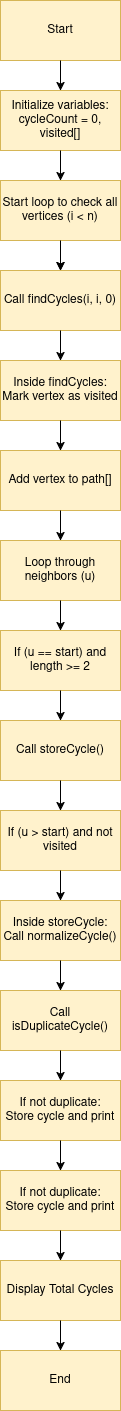
\includegraphics[width=0.2\columnwidth]{Caminhamento.png}  
    \caption{C Implementation: Traversal-based approach with adjacency matrix.}
    \label{fig:c_impl}
\end{figure}

\textbf{C++ implementation:} The permutation-based approach using an adjacency list.

\begin{figure}[H] % Adicionando [H] para fixar a posição
    \centering
    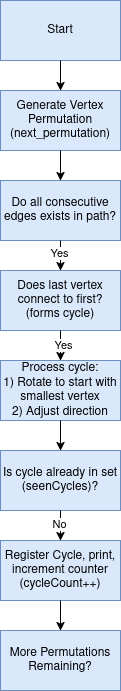
\includegraphics[width=0.2\columnwidth]{Permutacao.png}  
    \caption{C Implementation: Traversal-based approach with adjacency matrix.}
    \label{fig:cpp_impl}
\end{figure}


These implementations provide a practical evaluation of the theoretical concepts discussed earlier. The source codes are provided for reference and experimentation, allowing further testing and optimization.

\section{Performance Analysis}

To evaluate the efficiency of both approaches, we conducted a series of experiments measuring execution time and memory consumption for graphs of varying sizes and densities. The results indicate that:
\begin{itemize}
    \item The traversal-based approach is significantly more efficient for sparse graphs, as it does not need to generate all possible vertex orderings.
    The permutation-based approach becomes computationally infeasible for large graphs due to its factorial complexity. The results for the permutation approach were 35, while the traversal approach resulted in 38, being the correct one.
    \item The execution time for the permutation approach was 1540 microseconds, whereas the traversal approach executed in 343 microseconds, demonstrating its efficiency.
    \item The adjacency list representation is more memory-efficient than the adjacency matrix, particularly for large sparse graphs.
\end{itemize}

These findings highlight the importance of choosing the right algorithm based on the graph’s characteristics.
\section{Discussion}

If the graph were directed, the cycle enumeration process would require modifications to account for the directionality of edges. The key adaptations include:

\textbf{Traversal-Based Approach Adjustments:} The DFS algorithm would need to track edge directions and ensure that cycles respect the directed nature of the graph. This requires additional handling of directed back edges.

\textbf{Permutation-Based Approach Adjustments:} The algorithm must ensure that generated cycles follow the correct edge direction rather than arbitrarily forming loops.

While both methods can be adapted for directed graphs, the complexity of handling directionality makes traversal-based approaches more suitable for practical applications.

\section{Conclusion}

This study compared two methods for cycle enumeration in undirected graphs, highlighting their computational complexity, efficiency, and practical considerations. The permutation-based approach, while theoretically exhaustive, is computationally prohibitive for large graphs. In contrast, the traversal-based approach is significantly more efficient, particularly for sparse graphs. Future work could explore further optimizations, such as parallel processing techniques or hybrid methods combining aspects of both approaches to enhance performance.

\cite{ref1}
\cite{ref2}
\cite{ref3}

\printbibliography[title={References}]

\end{document}

